\documentclass[portrait,final]{baposter} % final version
%\documentclass[a4shrink,portrait]{baposter} % draft (some conferences request a shrink version for review)

\tracingstats=2

%\usepackage{pgfbaselayers} % deprecated
\pgfdeclarelayer{background}
\pgfdeclarelayer{foreground}
\pgfsetlayers{background,main,foreground}
\newcommand{\captionfont}{\footnotesize}

%% Load custom packages
%% ----------------------------------------------------------------------------
%% Load poster packages and optionally define your custom commands
%%
% The hyperref package does not work (the author is aware of this)
%%

\usepackage{calc}
\usepackage{amsmath}
\usepackage{amssymb}
\usepackage{relsize}
\usepackage{bm}
\usepackage{url} 

\usepackage{shortvrb}
\MakeShortVerb{\|}

\usepackage{times}
\usepackage{helvet}
%\usepackage{bookman}
\usepackage{palatino}

\usepackage{graphicx}
\graphicspath{{logos/},{images/}}
\usepackage{xcolor}
\usepackage{colortbl}

\usepackage{multicol}
\usepackage{multirow}
% Professional tables
\usepackage{booktabs}
\newcommand{\head}[1]{\textnormal{\textbf{#1}}}

% Multicol Settings
\setlength{\columnsep}{0.7em}
\setlength{\columnseprule}{0mm}

% Save space in lists. Use this after the opening of the list
\newcommand{\compresslist}{
  \setlength{\itemsep}{1pt}
  \setlength{\parskip}{0pt}
  \setlength{\parsep}{0pt}
}

% A command to avoid indenting list items. Use this after the opening of the list
\newcommand{\noindentlist}{
  \setlength{\leftskip}{-1.5em}
}

%\usepackage[cmex10]{amsmath}
\usepackage{amsmath}
\DeclareMathOperator*{\argmax}{arg\,max}
\DeclareMathOperator*{\kbest}{k-best}
% \DeclareMathOperator*{\eqdef}{\stackrel{\mathsf{def}}{=}}
\DeclareMathOperator*{\eqdef}{\stackrel{\text{\tiny def}}{=}}

\DeclareMathOperator*{\w}{\mathbf{c}}
\DeclareMathOperator*{\vv}{\mathbf{c}_v}
\DeclareMathOperator*{\x}{\mathbf{x}}
\DeclareMathOperator*{\e}{\mathbf{e}}
\DeclareMathOperator*{\R}{\mathbf{R}}
\DeclareMathOperator*{\X}{\mathbf{X}}
\DeclareMathOperator*{\Q}{\mathbf{V}}
\DeclareMathOperator*{\W}{\mathbf{C}}

% Professional tables
\usepackage{booktabs}
\usepackage{array}

% To draw automata
\usepackage{tikz}
\usetikzlibrary{arrows,shapes,automata,positioning}


%% ----------------------------------------------------------------------------
%% set colors for later use in your baposter

% Base colors (always available, since the cls uses the xcolor package) are:
% black blue brown cyan darkgray gray green lightgray lime magenta olive orange pink purple red teal violet white yellow

% Defined colors in RGB space
\definecolor{pantone640rgb}{RGB}{80,171,202}
\definecolor{pantone647rgb}{RGB}{35,93,141}
\definecolor{pantone122rgb}{RGB}{254,226,127}
\definecolor{pantone1375rgb}{RGB}{249,173,28}
% Defined colors in CMYK space
\definecolor{pantone640cmyk}{cmyk}{0.6,0.15,0,0.21}
\definecolor{pantone647cmyk}{cmyk}{0.75,0.34,0,0.45}
\definecolor{pantone122cmyk}{cmyk}{0,0.11,0.50,0}
\definecolor{pantone1375cmyk}{cmyk}{0,0.31,0.89,0.2}

%------------------------------------------------------------------------------
% Colors
\definecolor{lightblue}{rgb}{0.145,0.6666,1} % Defines the color used for content box headers
\definecolor{lightred}{rgb}{0.941,0.678,0.337} % Defines the color used for content box headers
\definecolor{darkred}{rgb}{0.6,0.1,0.1}
\definecolor{darkgreen}{rgb}{0.2,0.5,0.3}
\definecolor{greygreen}{rgb}{0.25,0.5,0.25}
\definecolor{darkblue}{rgb}{0.1,0.2,0.6}
\definecolor{titleblue}{rgb}{0.1,0.2,0.4}
\definecolor{palered}{rgb}{1.0,0.85,0.8}
\definecolor{blue5}{rgb}{0.0,0.2,0.3}
\definecolor{darkgreen}{rgb}{0.2,0.5,0.3}
\definecolor{LightCyan}{rgb}{0.88,1,1}
\newcommand{\dred}[1]{\textbf{\textcolor{darkred}{#1}}}
\newcommand{\red}[1]{\textbf{\textcolor{red}{#1}}}
\newcommand{\dblue}[1]{\textbf{\textcolor{darkblue}{#1}}}
\newcommand{\tblue}[1]{\textcolor{titleblue}{#1}}
\newcommand{\blue}[1]{\textbf{\textcolor{blue}{#1}}}
\newcommand{\mblue}[1]{\textcolor{blue5}{#1}}
\newcommand{\pred}[1]{\textcolor{palered}{#1}}
\newcommand{\dgreen}[1]{\textcolor{darkgreen}{#1}}
\newcommand{\ggreen}[1]{\textbf{\textcolor{greygreen}{#1}}}
%------------------------------------------------------------------------------

\selectcolormodel{cmyk}

%% ----------------------------------------------------------------------------
%% Poster (5) options: settings, title, author(s), eyecather image, and logos
%%

\def\posterconfig{
	%\input{poster-theme}
	% cannot load poster settings from a separate file... (keyval error) -- must be set in poster.tex
}

\def\postertitle{\vspace{.2em}
  %\centering
  \hspace{-.7em}%
  \begin{minipage}[b]{.25\linewidth}
   \raisebox{.45em}{ 
    
\includegraphics[width=\linewidth]{Khoury_logo}}
  \end{minipage}%\hspace{-.8em}%
  \raisebox{.6em}{
    \begin{minipage}[b]{.58\linewidth}
      \centering
      \bf{\huge Digital Editions as Distant Supervision\\[-.3em]
        for Layout Analysis of Printed Books}
    \end{minipage}}%\hspace{.01\linewidth}%
  \begin{minipage}[b]{.15\linewidth}
    %
\includegraphics[height=2.1em]{OpenITI_logo}\hspace{.3em}%
    \raisebox{.4em}{
    
\includegraphics[width=\linewidth]{Mellon-Logo}}
  \end{minipage}
}

\def\posterauthor{\vspace{-.5em}%
  \hspace{4em}Alejandro H. Toselli, Si Wu, and David A. Smith
}

\def\postereyecatcher{
	\includegraphics[height=8em]{D1077.png} % only shown if eyecatcher=yes
	% If an eye catcher image is present, the title floats at the left margin of such image
    % To adjust position you can use the following strategy:
    %\raisebox{4em}{ % the vertical offset
    %  \begin{minipage}[t]{5.5em} % the horizontal offset
	%	\includegraphics[height=5em]{image} % the image height
    %  \end{minipage}
	%}
}

\def\posterlogos{
	% Look inside 'logos' dir for alternative logo formats, 
	% or browse the PRHLT logos SVN repository:
	% https://svn.prhlt.upv.es/documentation/logos/pdf/
  % \mbox{
  %   \begin{minipage}[c]{8.6em}
  %     \includegraphics[height=3em]{logoUPV-val-horizontal}
  %   \end{minipage}
  % }
  %
  \mbox{
    \begin{minipage}[c]{10.2em}
      
\includegraphics[height=3em]{Khoury_logo2}
    \end{minipage}
  }%
  \hspace{3em}
  \mbox{
    \begin{minipage}[c]{4.2em}
      
\includegraphics[height=3em]{OpenITI_logo}
    \end{minipage}
  }%
  \hspace{1em}
  %
  \mbox{
    \begin{minipage}[c]{4.2em}
      
\includegraphics[height=3em]{Mellon-Logo}
    \end{minipage}
  }%
  % \mbox{
  %   \begin{minipage}[c]{4.2em}
  %     \includegraphics[height=3em]{READ_text_bottom}
  %   \end{minipage}
  % }
}


\begin{document}

\background{ % used only if background=user
  \begin{tikzpicture}[remember picture,overlay]
    \draw (current page.north west)+(-2em,2em) node[anchor=north west] {\includegraphics[height=1.1\textheight]{silhouettes-background}};
  \end{tikzpicture}%
}
\newlength{\leftimgwidth}

\begin{poster}%
  {
    grid=no,                            % show grid (to help with alignment)
    gridColumns=3,                      % number of columns for use in grid (e.g., you can set 3 columns on portrait mode and 4 for landscape)
    colspacing=1.5em,                   % column spacing
    eyecatcher=no,                      % enable eye catcher (or not)
    %
    % Color styles
    %bgColorOne=white,                   % background top color
    bgColorOne=pantone122cmyk,                   % background top color
    %bgColorTwo=pantone122cmyk,          % background bottom color
    bgColorTwo=white,          % background bottom color
    %borderColor=pantone647cmyk,         % outer border color of poster units (boxes)
    borderColor=black,              % outer border color of poster units (boxes)
    %headerColorOne=pantone647cmyk,      % box header color
    headerColorOne=black,               % background color for the header in the content boxes (left side)
    %headerColorTwo=white,               % used if shades are enabled
    headerColorTwo=lightblue,           % background color for the header in the content boxes (right side)
    headerFontColor=white,              % box title color
    boxColorOne=white,                  % box background
    boxColorTwo=white,                  % used if shades are enabled
    %
    % Format of text header
    textborder=roundedleft,             % type of box border
    headerheight=0.09\textheight,      % set poster size relative to poster title height (as the title can be too long)
    headershape=roundedright,           % shape of the box-header region
    headerborder=open,                  % no extra border above box header
    headershade=shade-lr,               % type of box-header shading
    %headerfont=\Large\sf,               % header font
    %textfont=\sf,                       % text font
    boxshade=plain,                     % box shading
    background=shade-tb,                % type of poster background
    linewidth=1pt                       % border for all boxes
  }
  {
    \postereyecatcher
  }
  {
    \postertitle
  }
  {
    \posterauthor
  }%
  %{
  %  \posterlogos
  %}%

  % set some shading options, once the poster is already configured
  %\tikzstyle{light shaded}=[top color=baposterBGtwo!30!white,bottom color=baposterBGone!30!white,shading=axis,shading angle=30]

  %% ----------------------------------------------------------------------------
%% Define your poster sections
%%
% Each box is defined as \headerbox{title}{options}{content}
% Box options are the following:
% name=   [noname] box name, for later referencing
% column= [0]      column index
% row=    [0]      row index
% span=   [1]      column span
% height= [auto]   size in percent of column height
% below=           name of other node
% above=           name of other node
% aligned=         name of other node
% bottomaligned=   name of other node
%%

% % -----------------------------------------------------------------------------
% \headerbox{Acknowledgments}{name=ack,column=0,span=3,above=bottom}{
% % -----------------------------------------------------------------------------
%   \small%
%   Work partially supported by ...
% }
  

% -----------------------------------------------------------------------------
\headerbox{1. Introduction}{name=intro,column=0,row=0}{
% -----------------------------------------------------------------------------
  \begin{itemize}
    % \compresslist
    \itemsep=-.0em
    \small 
    \setlength{\leftskip}{-1.5em}

  \item Data for training/evaluating LA models %on page images
    are usually produced by manual annotations.

  \item Other sources of information to retrieve such data:
    \dred{digital editions with semantic markup}.
    
  \item Such editions
    %with semantic markup
    use XML to record logical \& physical components: title,
    body, ln-brks, \ldots
    %notes and figures, page and line
    %breaks, etc.

  \item A common markup scheme: %''Text Encoding Initiative´´
    \dred{TEI}. It
    %use for representing such features of textual resources and
    abstracts away from the precise appearance information.

  \item Present Methods for exploiting this semantic markup as distant
    supervision for training \& evaluating LA models.
    
  \end{itemize}
  %\vspace{-.5em}
}

% -----------------------------------------------------------------------------
\headerbox{2. Analyzing GT Markup}{name=markup,column=0,below=intro}{
% -----------------------------------------------------------------------------
  \begin{itemize}
    % \compresslist
    \itemsep=-.0em
    \small 
    \setlength{\leftskip}{-1.5em}

  \item Top-level units of layout are \dred{regions} containing
    figures or text lines with specific reading order.
    % (top-to-bottom and left-to-right).
        
  \item Consider eight region types:\\[.7em]
    % body, caption, catchword, figure,
    % note, pageNum, signature, title.
    \centerline{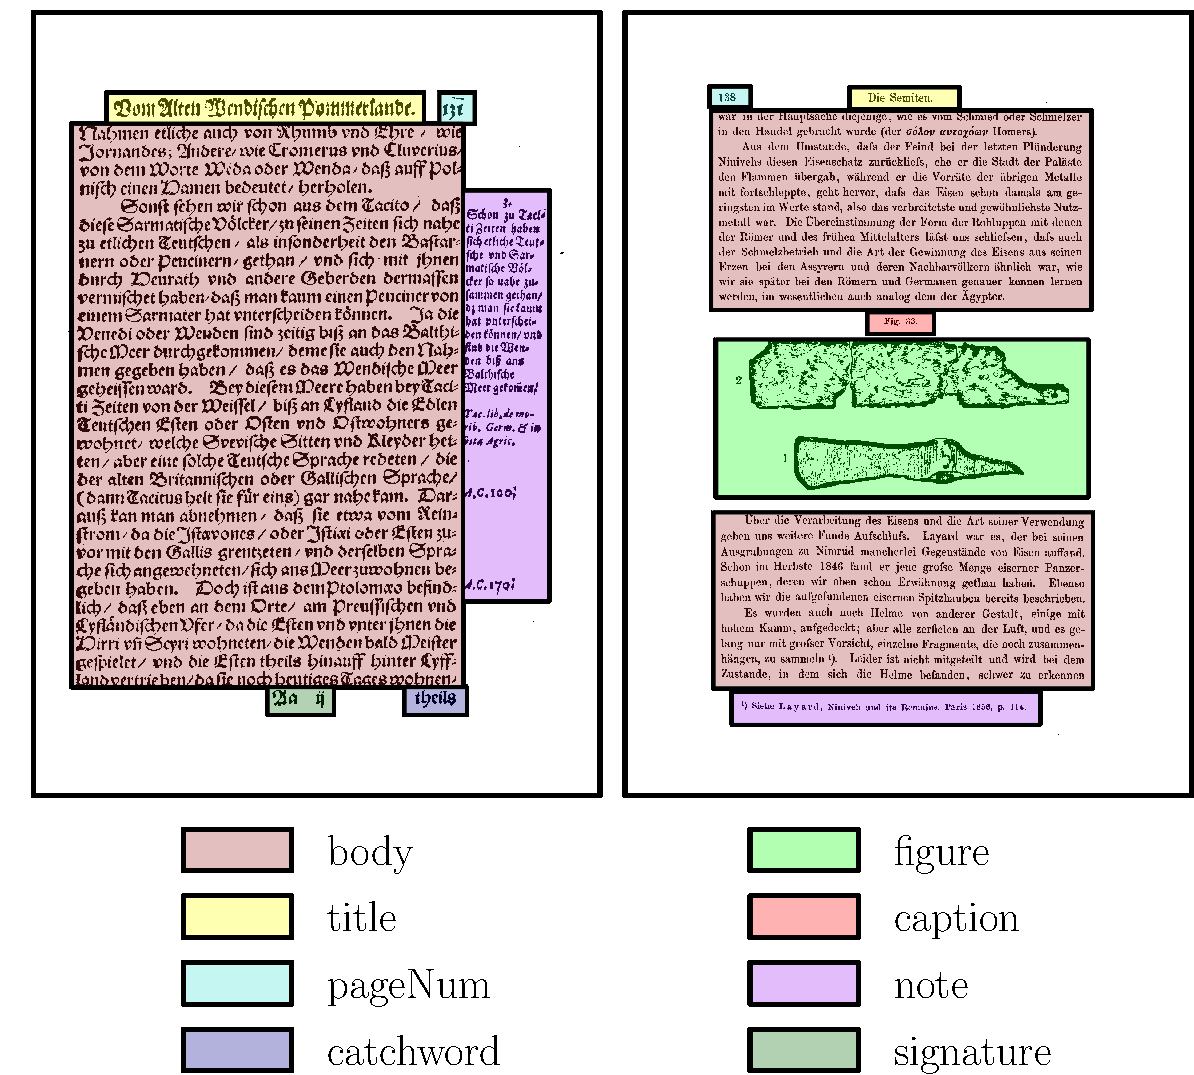
\includegraphics[width=.83\linewidth]{RegionTypes/regionTypes}}

  \item The different region types do not hold necessarily a specific
    reading order on a page.
        
  \item The encoding conventions of these regions are analyzed in
    three corpora of historical books:\\[-2em]
    \begin{enumerate}
      \itemsep=-.0em
      \small 
      \setlength{\leftskip}{-2.5em}
    \item \dred{Deutsches Textarchiv (DTA)}: with transcripts of 1406
      German books.% encoded in TEI XML.
    \item \dred{The Women Writers Online (WWO):} 336 books
      % of womens' writing
      in English % transcribed in TEI XML but
      without page images.% in the edition transcribed.
    \item \dred{Text Creation Partnership (TCP)}: % containing TEI XML
      32,853 transcribed books from %propietary
      microfilm series.
    \end{enumerate}
    \vspace{-.5em}%
    %\begin{center}
    %  \includegraphics[height=.35\linewidth]{Examples/DTA_0160}\hspace{1em}%
    %  \includegraphics[height=.35\linewidth]{Examples/WWO_0019}%\hspace{1em}%
      % \includegraphics[height=.35\textwidth]{Examples/TCP_xxxx}
    %\end{center}

  \item Summary of page zone markup in TEI editions from the 3 corpora:
    \begin{center}
      \vspace{-2em}
      \scalebox{.5}{
        \begin{minipage}{2\linewidth}
          \extrarowheight=3pt
          \begin{tabular}{>{\bf}l|l|l}
            \hline
            \rowcolor{lightgray}
            \bf Corpus & \bf Caption & \bf Catchword \\
            \hline
            DTA & //figure/* & //fw[\@type='catch'] \\
            TCP & //figure/*[not(self::figDesc)] & --- \\
            WWO & //figure/*[not(self::figDesc)] & //mw[@type='catch'] \\
            \cline{2-3}
                       & \cellcolor{lightgray}\bf Column head & \cellcolor{lightgray}\bf Figure \\ \hline
            DTA & //cb[substring(@n,1,1)!='[']/@n & //figure \\
            TCP & --- & //figure \\
            WWO & --- & //figure \\
            \cline{2-3}
                       & \cellcolor{lightgray}\bf Note &  \cellcolor{lightgray}\bf Pagination \\ \hline
            DTA & //note & //pb[substring(@n,1,1)!='[']/@n \\
            TCP & //note & --- \\
            WWO & //notes/note & //mw[@type='pageNum'] \\
            \cline{2-3}
                       & \cellcolor{lightgray}\bf Running title & \cellcolor{lightgray}\bf Signature \\ \hline
            DTA & //fw[@type='head'] & //fw[@type='sig'] \\
            TCP & --- & --- \\
            WWO & --- & //mw[@type='sig'] \\
            \hline
          \end{tabular}
        \end{minipage}}
    \end{center}

  \item \dred{Body text} is defined as all content
    % of the <text> element
    that are not described by one of the elements in Table above.
    
  \item \dred{DTA \& WWO} transcribe printed page numbers. DTA also
    transcribes
    % running
    titles
    % at the top of pages
    and column heads.
    
  % \item DTA \& TCP insert <note> elements near reference marks printed
  %   in the body for foot-/end-notes. The WWO transcribed all notes
  %   in a separate section, where each child note is linked by using an
  %   XML IDREFs.
    
  %\item \dred{DTA \& TCP} insert <note> elements near reference marks printed
  %  in the body for foot-/end-notes. The \dred{WWO} transcribed all notes in
  %  a separate section.
  \item The three corpora transcribe notes (marginal and foot-/end notes).

  % \item Foot-/end-notes continue onto the next pages. So each part of
  %   the text of these run-on notes is associated with the
  %   corresponding page.

  \item \dred{DTA \& WWO} also record line breaks, and \dred{TCP} does not. 
  %\dred{Body text} might be broken into different zones by page and line breaks.

  \item Because its consistently encoding, \dred{DTA} was used for
    bootstrapping annotated data for LA.
    
  \item A page-level aligned subset of \dred{WWO} was compiled to test the
    generalization of layout models trained on \dred{DTA}.

  \item As \dred{TCP} transcribes a few of the main page regions, it was not included in the experiments.

  \end{itemize}
  
  \vspace{-.5em}
}

  
% -----------------------------------------------------------------------------
\headerbox{3. Annotation by FA}{name=forceAlign,column=1,bottomaligned=intro}{
% -----------------------------------------------------------------------------
  \begin{itemize}
    % \compresslist
    \itemsep=-.0em
    \small 
    \setlength{\leftskip}{-1.5em}
  
  \item For training/evaluating layout models, we need to link digital
    editions to page images.

  \item Image annotations at page/pixel-level produced by
    force-alignment between the digital edition text and the output
    text of a baseline OCR.
    
  \item %Most LA model evaluations
    Pixel-level layout evaluation require assigning
    rectangular/polygonal zones to regions.
  
  \item For page-level annotation, \dred{DTA} already links images to each
    page of its 1,406 XML editions.
    
  % \item WWO page-level alignment, using PASSIM text-reuse analysis
  %   system, 336 XML editions were aligned with a corpus of 347,428
  %   OCR'd (ABBYY FineReader) early modern books from the Internet
  %   Archives (IA). After the process, 23 books were selected which
  %   80\% of the pages aligned with IA.
    
  \item Page-level annotated 23 books (3,549p.) selected from \dred{WWO} after
    aligning their 336 XML editions with a corpus of 347,428 OCR'd
    books.% (ABBYY F.). early modern books from the Internet
                % Archives.
    
  \end{itemize}
}

% -----------------------------------------------------------------------------
\headerbox{4. Figure Region Detection}{name=figDet,column=2,bottomaligned=forceAlign}{
% -----------------------------------------------------------------------------
  \begin{itemize}
    % \compresslist
    \itemsep=-.0em
    \small 
    \setlength{\leftskip}{-1.5em}

  \item In the considered digital editions, figures are not annotated
    with their exact coordinates or sizes.
    
  \item F-RCNN based pretrained model: 
  %\dred{PubLayNet} and
    \dred{Newspaper Navigator} was used to detect figures.

  \item \dred{Newspaper Navigator} was ran on all page images whose GT
    had the \texttt{<figure>} element.
    
  %\item The detected figures sometimes include parts of other elements
  %  such as caption or body text.% near the figure.

  \end{itemize}
}
    
% -----------------------------------------------------------------------------
\headerbox{5. Pixel-level Text Region Annotation on Page Images}{name=textRegAlign,column=1,span=2,below=forceAlign}{
% -----------------------------------------------------------------------------
  {\small
    For pixel-level annotation, we require region locations on the
    physical images. Steps carried out:}
  \vspace{-.3em}
    \begin{enumerate}
      % \compresslist
      \itemsep=-.0em
      \small 
      \setlength{\leftskip}{-1em}
    \item \dred{Tesseract OCR system} was run on all DTA page images using its
      publicly pretrained German model.
    % \item OCR output is the aligned with the the GT transcripts of the
    %   DTA XMLs in two steps: first we use PASSIM to perform line-level
    %   alignment of the OCR output with the DTA text; then, a
    %   fine-grain character-level force alignment was applied between
    %   of the remaining no-yet-aligned OCR output (and the already
    %   aligned text) with the GT text to correct possible aligned
    %   segmentataion issues for which PASSIM failed due to the limited
    %   textual context (page and column numbers, signatures, short
    %   titles, catchwords, etc.)
      
    \item \dred{PASSIM} used to get a coarse line-level alignment of
      OCR'd page texts and corresponding DTA XMLs.
    \item A \dred{fine-grained character-level FA} was applied between the
      remaining no-yet-aligned OCR output (including the already
      aligned one) with the DTA XML text to correct possible aligned
      issues.
      % segmentataion issues
      
    % \item Regions boundaries can be inferred from bounding boxes of
    %   OCR's text lines.  Assuming region transcripts are in RO, we
    %   combine in that order all OCR line BBs and the boundary of the
    %   resulting combination is taken as that of the region.

    \item \dred{Regions boundaries} were obtained by combining bounding boxes
      of their OCR's text lines, which are assumed to be in reading
      order.
      
    \item Finally, a subset of 454 pages with correct aligned regions
      was selected by visual inspection.
    \end{enumerate}
    \vspace{-1em}%
    % 
    \begin{center}
    \begin{minipage}[t]{.2\textwidth}
      \centering
      \setlength{\fboxsep}{0pt}
      Page to Align\\
      \fbox{
      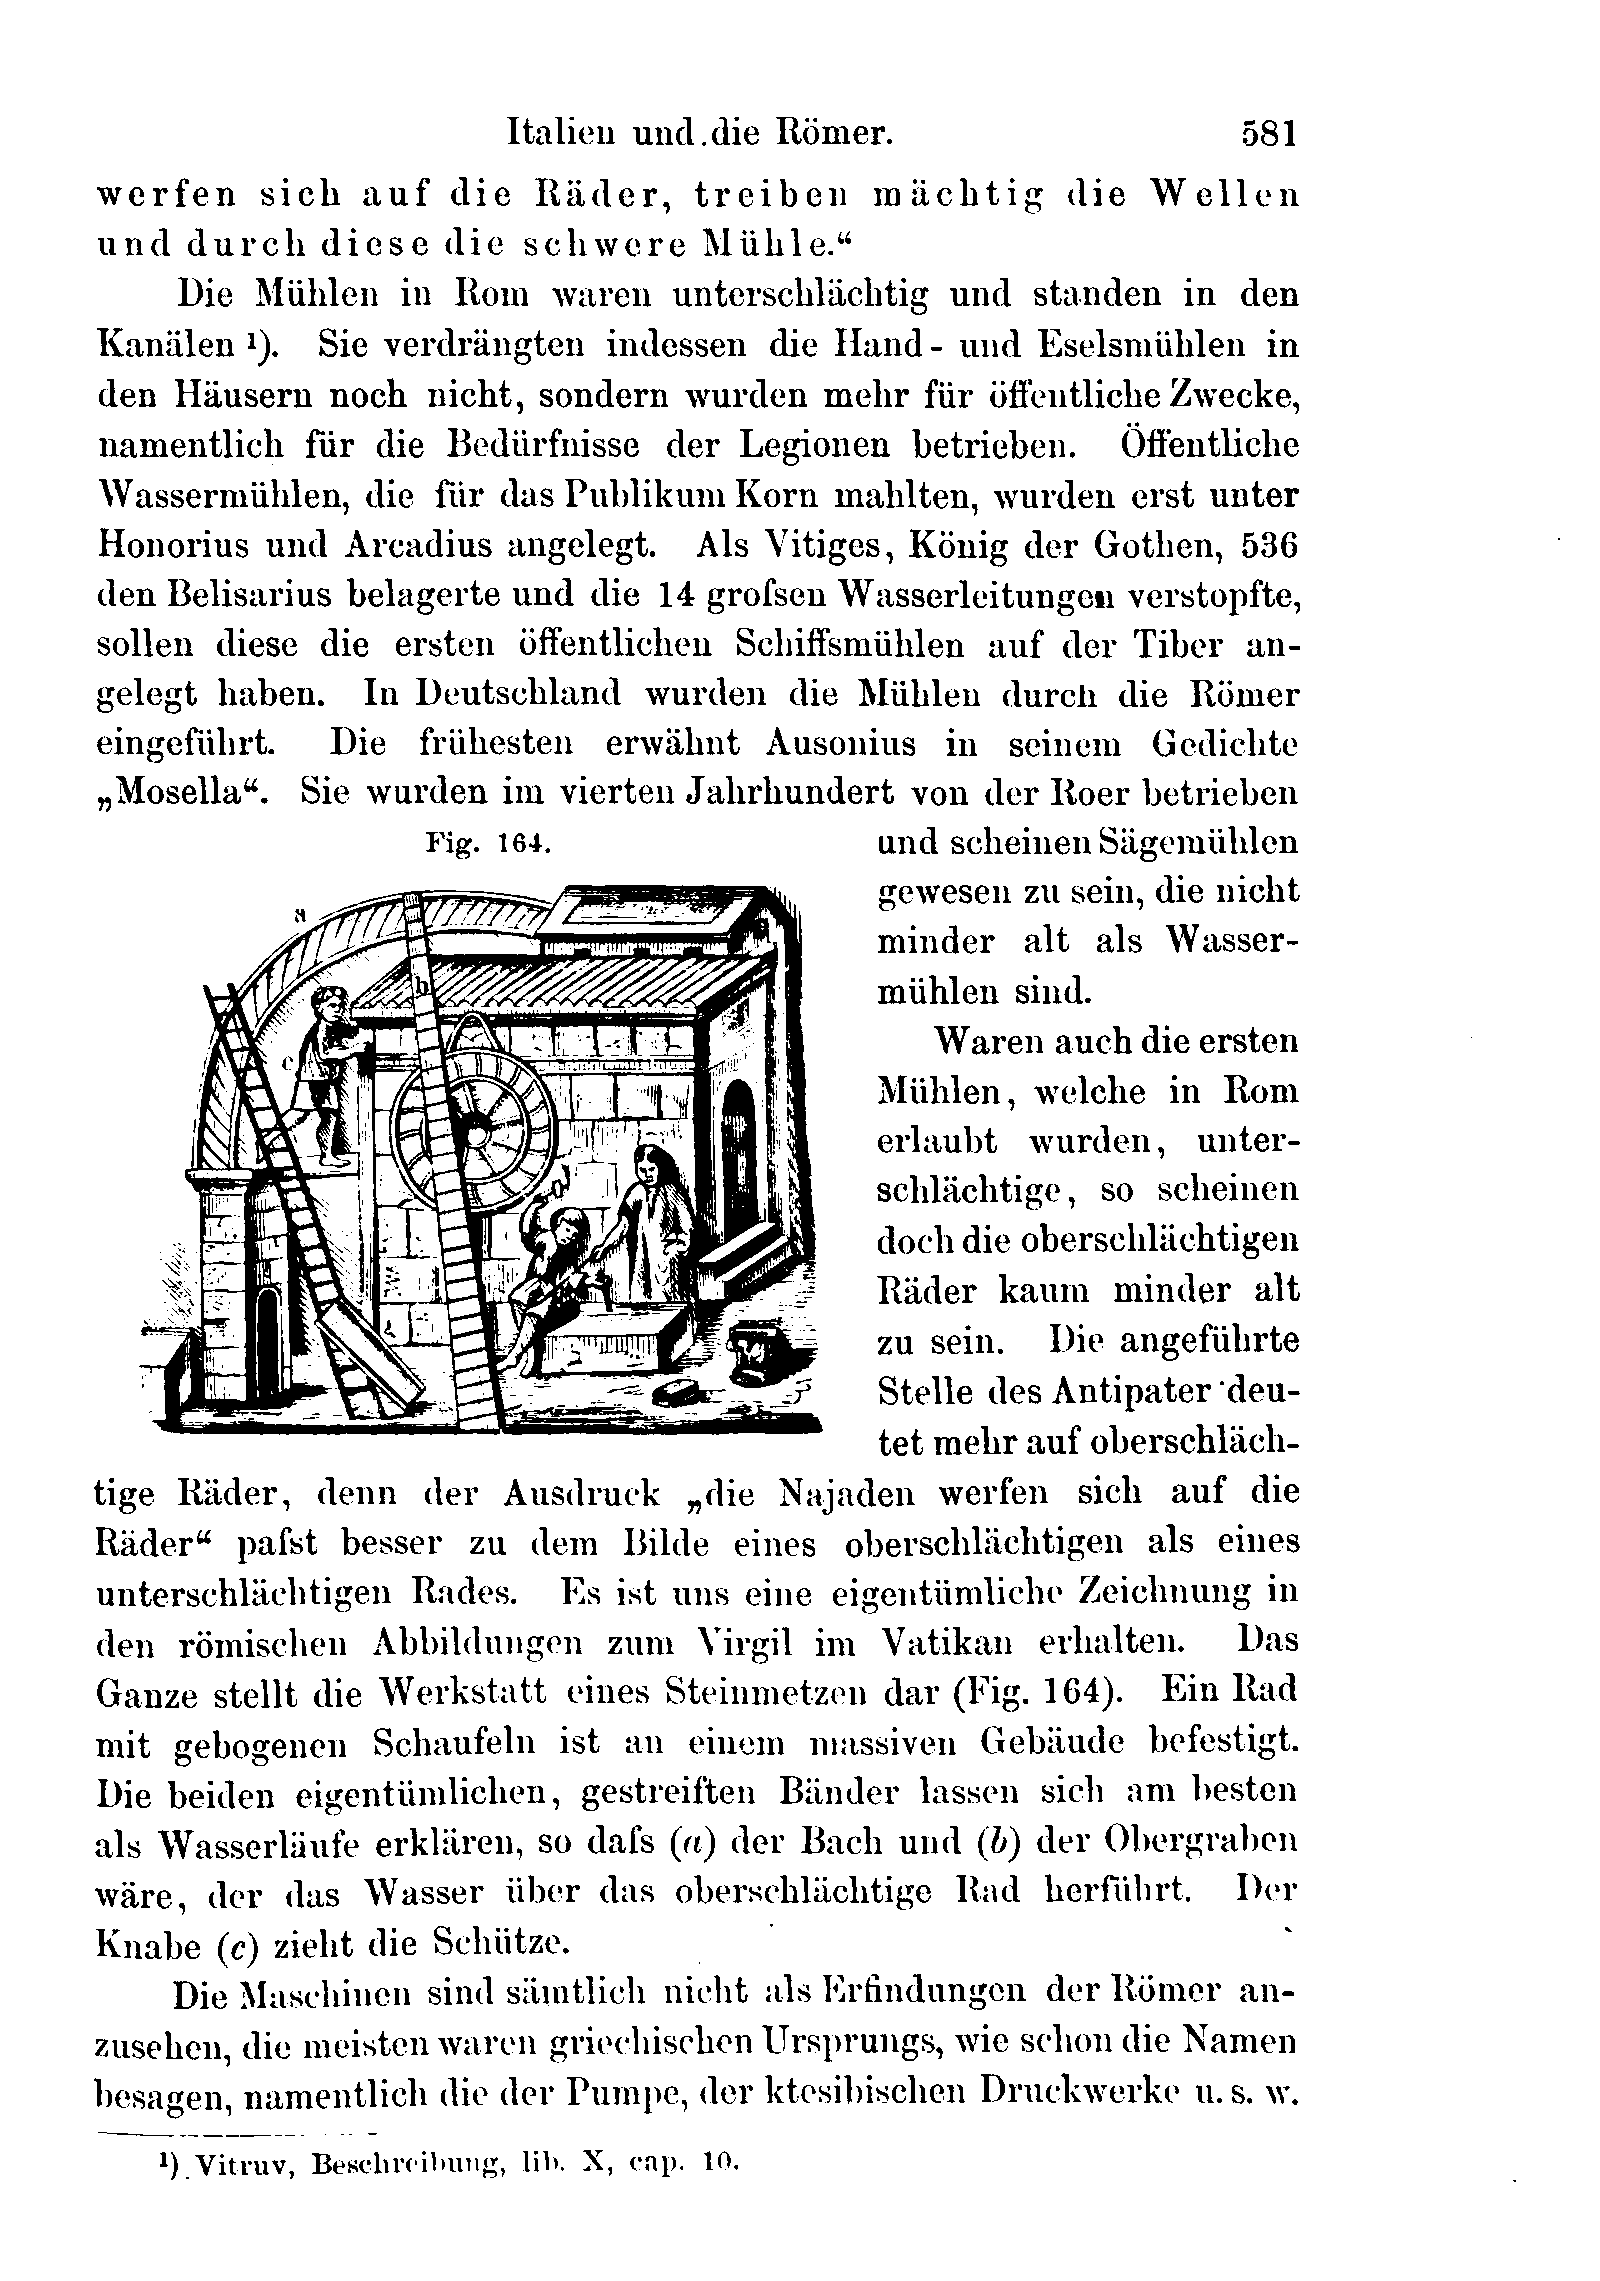
\includegraphics[width=\textwidth]{coarseGrained-FA/0603_crop.png}}
    \end{minipage}\hspace{.5em}%
    \begin{minipage}[t]{.2\textwidth}
      \centering
      \setlength{\fboxsep}{0pt}
      PASSIM FA\\[.26em]
      \fbox{
      \includegraphics[width=\textwidth]{coarseGrained-FA/0603_dsp_woFig_crop.png}}
    \end{minipage}\hspace{.5em}%
    \begin{minipage}[t]{.2\textwidth}
      \centering
      \setlength{\fboxsep}{0pt}
      Fine-grained FA\\
      \fbox{
      \includegraphics[width=\textwidth]{fineGrained-FA/0603_dsp_woFig_crop.png}}
    \end{minipage}\hspace{1.5em}%
    %\begin{minipage}[t]{.2\textwidth}
    %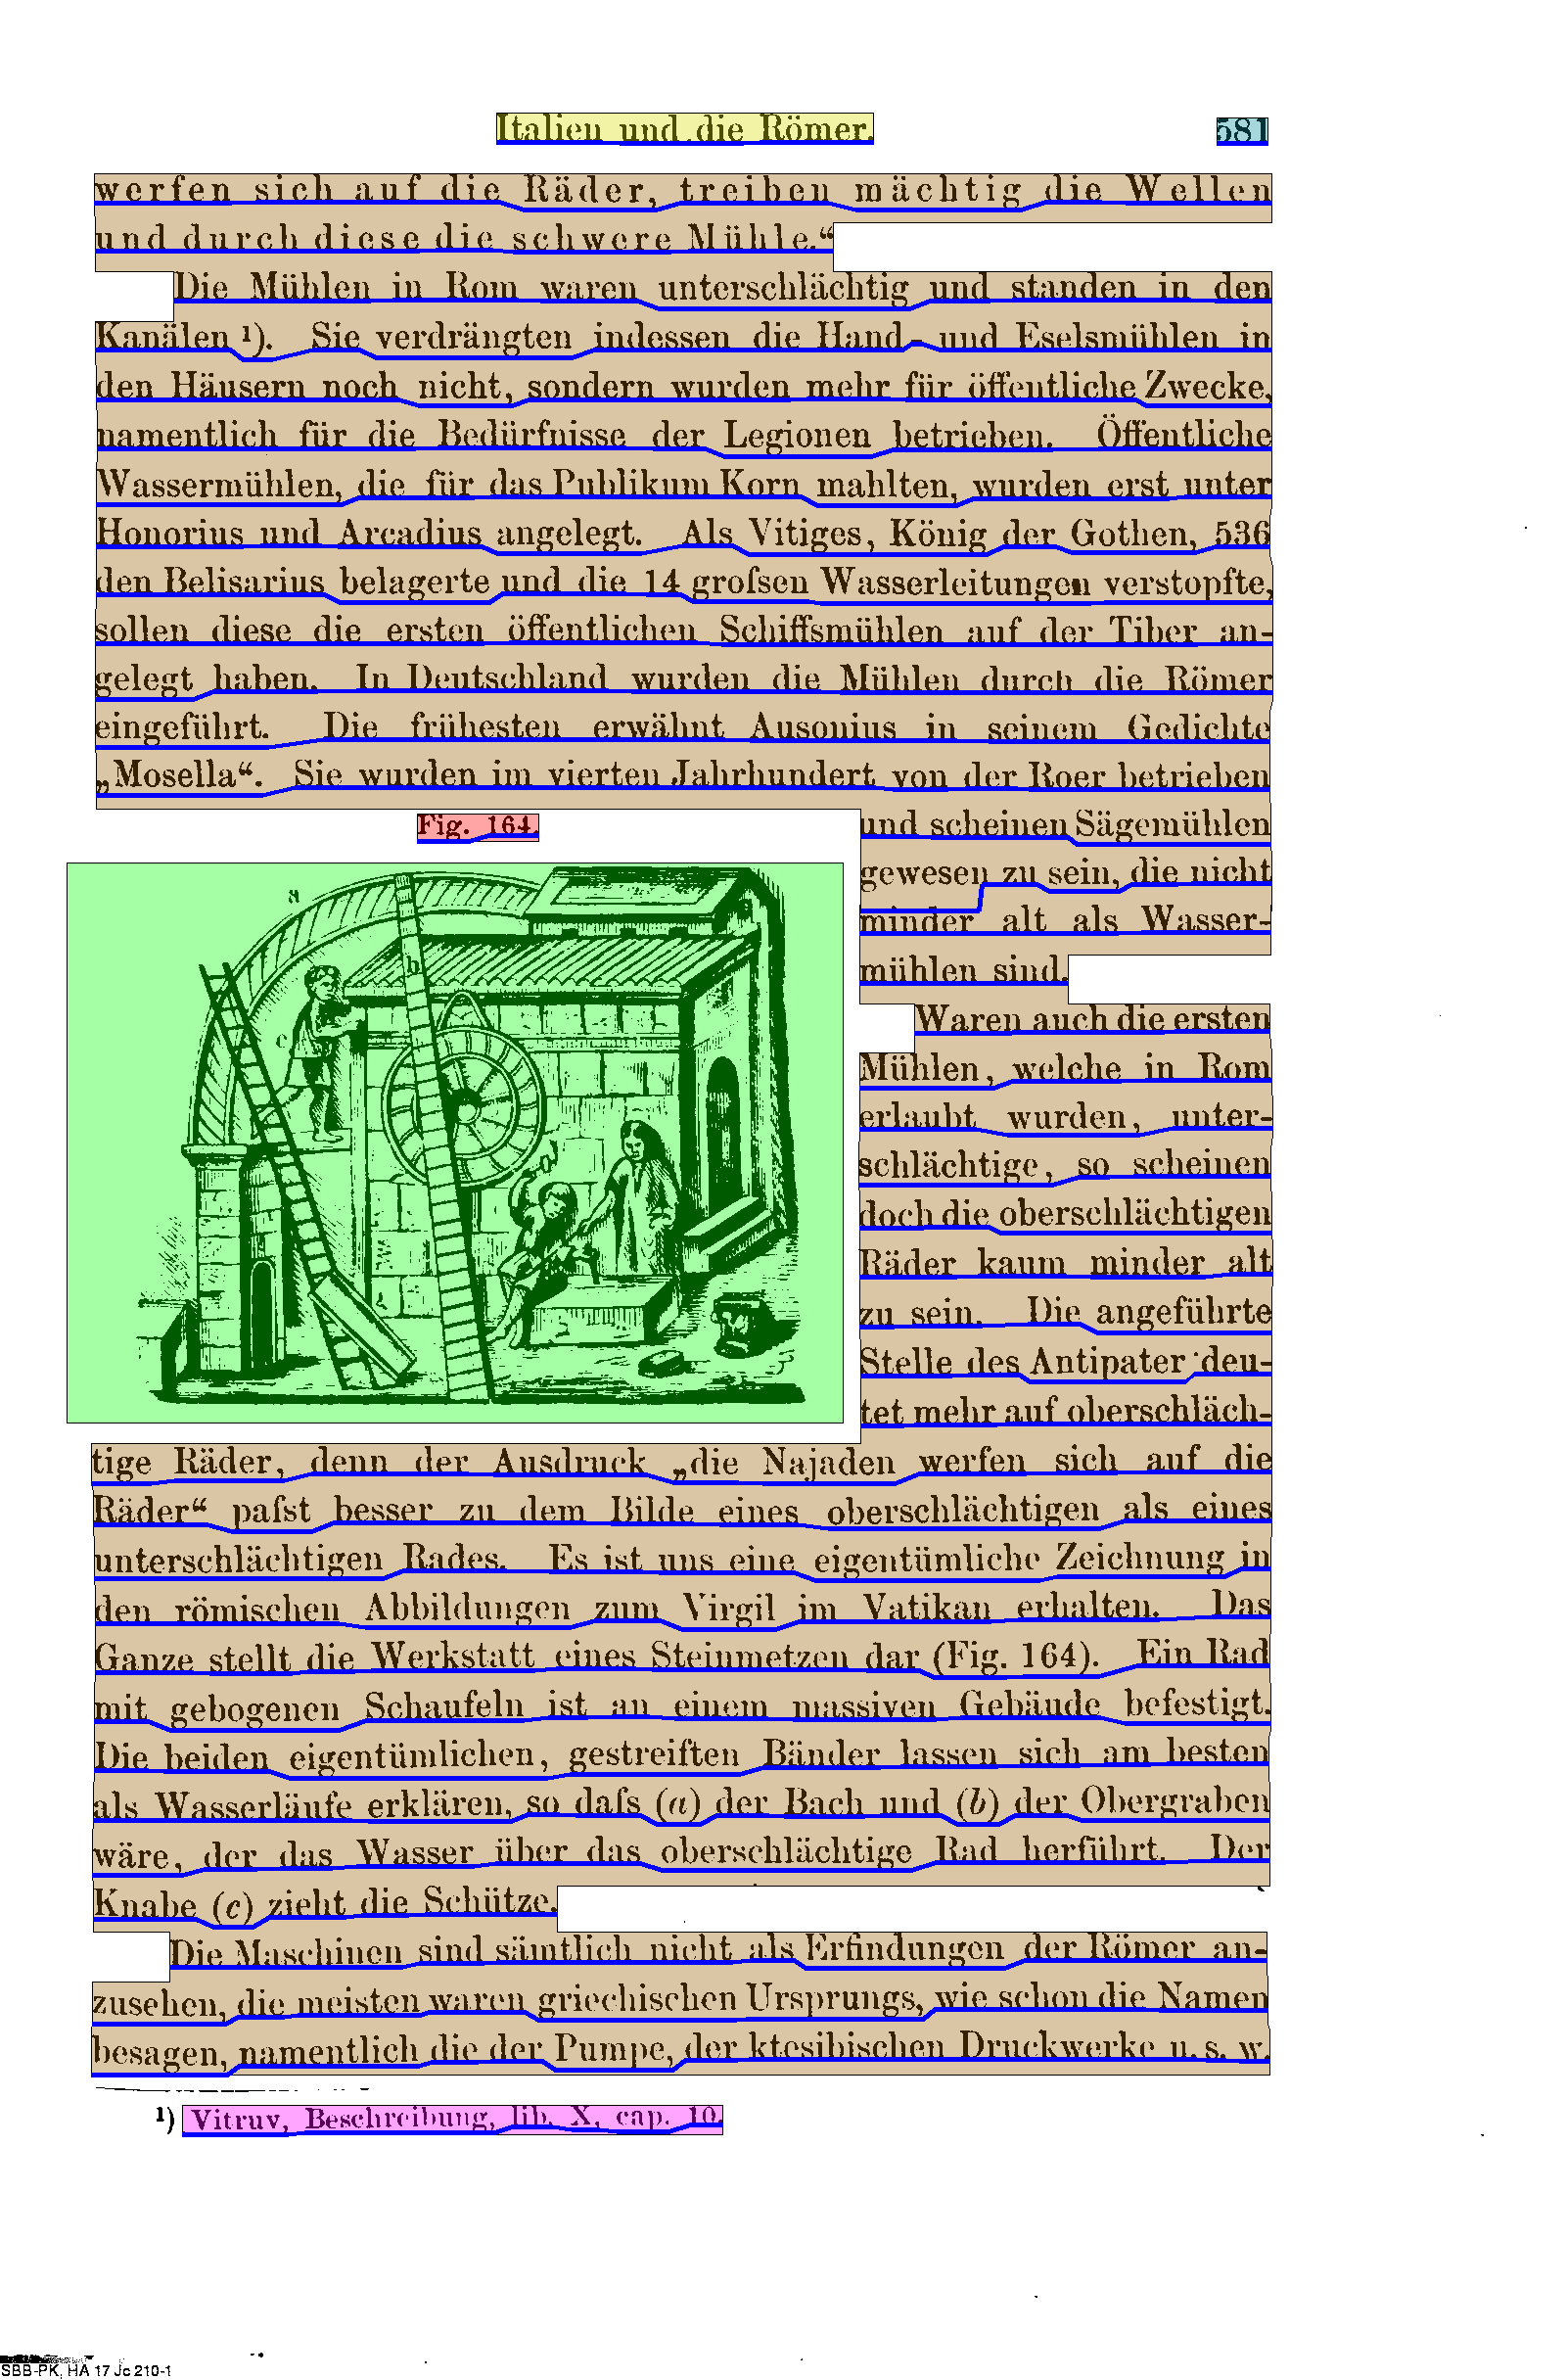
\includegraphics[width=\textwidth]{fineGrained-FA/0603_dsp.png}
    %\end{minipage}
    \begin{minipage}[t]{.25\textwidth}
      \centering
      Subset of selected pages:\\[.5em]
      {\scriptsize
      \begin{tabular}[t]{>{\bf}l|rr}
        % \toprule
        Region Type & Train & Test \\
        \midrule
        pages       &  318  &  136 \\
        \midrule
        body        &  340  &  146 \\
        caption     &   33  &   11 \\  
        catchword   &   17  &    4 \\   
        figure      &   53  &   23 \\ 
        note        &  318  &  125 \\
        pageNum     &  313  &  135 \\  
        signature   &   33  &   22 \\    
        title       &  279  &  122 \\
        % Total       & 1,386 &  588 \\
        \bottomrule
      \end{tabular}}
    \end{minipage}
    \end{center}
 
    \vspace{-.5em}
}

% -----------------------------------------------------------------------------
\headerbox{6. Predicted Region Evaluation by Region Types}{name=exp,column=1,row=2,span=2,below=textRegAlign,bottomaligned=markup}{
  \begin{itemize}
    % \compresslist
    \itemsep=-.0em
    \small 
    \setlength{\leftskip}{-1.5em}
    
  \item \dred{Pixel-level Evaluation:} F-RCNN, Kraken \& U-net trained
    on DTA data, and PubLayNet fine-tuned on it.
    %
    Polygonal annotat. were used with Kraken \& U-net, while
    rectangular with F-RCNN (and PubLayNet).
    % PubLayNet does
    % not output region types not in its original training data;
    % Kraken
    % produces no output for the smaller regions.

  \item \dred{Word-level Evaluation:} U-net predicted region
    performance evaluated through OCR output token positions by
    considering how many words of the ref. region fall inside/outside
    the pred. region boundary.
    
  \item \dred{Region-level Evaluation:} Consider whether the predicted
    regions are or not in the page ground-truth. U-net \& F-RCNN
    models trained on the 318-pages from DTA were used to perform this
    evaluation on the entire DTA and WWO collections: 519,362 and 3,549 pages respectively.
  \end{itemize}
  \vspace{-1.3em}

  \begin{center}\tiny
    %Pixel Level\hspace{}Word Level\hspace{}Region Level\\
    \tabcolsep=2pt
    % \extrarowheight=2pt
    \begin{tabular}[t]{l|rr|rr|rr|rr}
      \multicolumn{1}{c}{} & \multicolumn{8}{c}{\scriptsize Pixel Level} \\[.2em]
      \toprule
      \multirow{3}{*}{Region type}  & \multicolumn{2}{c}{PubLayNet} & \multicolumn{2}{c}{F-RCNN} & \multicolumn{2}{c}{Kraken} & \multicolumn{2}{c}{U-net} \\
        & \multicolumn{2}{c}{DTA} & \multicolumn{2}{c}{DTA} & \multicolumn{2}{c}{DTA} & \multicolumn{2}{c}{DTA} \\
                & p\_acc & iu & p\_acc & iu & p\_acc & iu & p\_acc & iu \\
      \midrule
      % BG        & 0.987 & 0.888 & 0.963 & 0.932 \\
      \rowcolor{LightCyan}
      body      & 0.96 & 0.92 & 0.97 & 0.94 & 0.93 & 0.91 & 0.96 & 0.94 \\
      caption   & ---  & ---  & 0.91 & 0.77 & ---  & ---  & 0.78 & 0.60 \\
      \rowcolor{LightCyan}
      catchword & ---  & ---  & 0.50 & 0.40 & ---  & ---  & 0.51 & 0.33 \\
      figure    & 0.99 & 0.90 & 0.98 & 0.89 & ---  & ---  & 0.94 & 0.74 \\
      \rowcolor{LightCyan}
      note      & ---  & ---  & 0.98 & 0.92 & 0.82 & 0.77 & 0.93 & 0.88 \\
      pageNum   & ---  & ---  & 1.00 & 0.86 & ---  & ---  & 0.94 & 0.68 \\
      % colNum    & --- & ---  & --- & --- \\
      \rowcolor{LightCyan}
      signature & ---  & ---  & 0.82 & 0.60 & ---  & ---  & 0.37 & 0.26 \\
      title     & 0.97 & 0.84 & 0.99 & 0.87 & ---  & ---  & 0.96 & 0.74 \\
      \bottomrule
    \end{tabular}%
    \hspace{1em}%
    \begin{tabular}[t]{rrr}
      \multicolumn{3}{c}{\scriptsize Word Level} \\[.2em]
      \toprule
      \multicolumn{3}{c}{U-net} \\
      \multicolumn{3}{c}{DTA} \\
      %Region &
                  Rc   & Pr   & F1   \\
      \midrule
      \rowcolor{LightCyan}
      % body      &
                  0.91 & 0.98 & 0.94 \\
      %caption   &
                  0.63 & 0.73 & 0.66 \\
      \rowcolor{LightCyan}      
      %catchword &
                  0.33 & 0.33 & 0.33 \\
      %figure    &
                  ---  & ---  & ---  \\
      \rowcolor{LightCyan}      
      %note      &
                  0.85 & 0.98 & 0.91 \\
      %pageNum   &
                  0.81 & 0.81 & 0.81 \\
      \rowcolor{LightCyan}      
      %signature &
                  0.26 & 0.44 & 0.31 \\
      %title     &
                  0.92 & 0.97 & 0.94 \\
      \bottomrule
    \end{tabular}%
    \hspace{1em}%
    \begin{tabular}[t]{rrr|rrr}
      \multicolumn{6}{r}{\scriptsize Region Level: Evaluated on\!} \\[.2em]
      \toprule
      \multicolumn{6}{c}{F-RCNN} \\
      \multicolumn{3}{c}{DTA} & \multicolumn{3}{c}{WWO} \\
      Rc &   Pr &   F1 &   Rc &   Pr &   F1 \\
      \midrule
      \rowcolor{LightCyan}
      0.92 & 1.00 & 0.96 & 0.99 & 1.00 & 0.99 \\
      0.06 & 0.88 & 0.80 &  --- &  --- &  --- \\
      \rowcolor{LightCyan}
      0.26 & 0.96 & 0.41 & 0.54 & 0.48 & 0.52 \\
      %0.81 & 0.84 & 0.82 &  --- &  --- &  --- \\
      0.59 & 0.32 & 0.41 & 0.50 & 0.00 & 0.00 \\
      \rowcolor{LightCyan}
      0.61 & 0.64 & 0.62 & 0.42 & 0.18 & 0.26 \\
      0.81 & 0.79 & 0.80 & 0.61 & 0.23 & 0.34 \\
      \rowcolor{LightCyan}
      0.12 & 0.85 & 0.21 & 0.13 & 0.14 & 0.13 \\
      0.52 & 0.78 & 0.54 &  --- & ---  &  --- \\
      % OVERALL  & 0.78  & 0.52  & 0.54 & 0.34 & 0.53 & 0.37 \\ 
      \bottomrule
    \end{tabular}%
    %\hfill%
    \begin{tabular}[t]{|rrr|rrr}
      \multicolumn{6}{l}{\scriptsize\!the entire DTA/WWO} \\[.2em]
      \toprule
      %\multirow{3}{*}{Reg. Type} &
              \multicolumn{6}{|c}{U-net} \\
              \multicolumn{3}{|c}{DTA} & \multicolumn{3}{c}{WWO} \\
                  Rc &   Pr &   F1 &   Rc &   Pr &   F1 \\
      \midrule
      \rowcolor{LightCyan}
      %body    &
                0.89 & 0.89 & 0.89 & 0.95 & 0.95 & 0.95 \\
      %caption &
                0.85 & 0.37 & 0.52 &  --- &  --- &  --- \\ 
      \rowcolor{LightCyan}     
      % catchword &
                0.89 & 0.63 & 0.74 & 0.77 & 0.52 & 0.62 \\
      %colNum  & 0.20 & 0.25 & 0.22 &  --- &  --- &  --- \\ 
      %figure  &
                0.77 & 0.81 & 0.79 & 0.53 & 0.43 & 0.48 \\
      \rowcolor{LightCyan}           
      %note    &
                0.97 & 0.97 & 0.97 & 0.84 & 0.84 & 0.84 \\
      %pageNum &
                0.96 & 0.68 & 0.80 & 0.98 & 0.45 & 0.61 \\
      \rowcolor{LightCyan}      
      %signature &
                0.65 & 0.48 & 0.56 & 0.32 & 0.25 & 0.28 \\
      %title   &
                0.97 & 0.69 & 0.81 &  --- &  --- &  --- \\ 
      \bottomrule
    \end{tabular}%
  \end{center}
  
  \begin{itemize}
    % \compresslist
    \itemsep=-.0em
    \small 
    \setlength{\leftskip}{-1.5em}
    
  \item \dred{Improving Performance with Self-training:} the new 757 training pages added were restricted to those where all their regions have been successfully detected.
  \end{itemize}

  \vspace{-2em}
  \begin{center}
    \begin{minipage}[t]{.22\linewidth}
      \vspace{.2em}
      \textbf{\small Measures:}
      \begin{description}
        % \compresslist
        \itemsep=-0em
        \scriptsize
        \setlength{\leftskip}{1em}
      \item[\dred{p\_acc:}] pixel accuracy
      \item[\dred{iu:}] mean Jaccard Index
      \item[\dred{Pr:}] precision
      \item[\dred{Rc:}] recall
      \item[\dred{F1:}] F-measure
      \end{description}
    \end{minipage}%
    \begin{minipage}[t]{.6\linewidth}
    \tiny
    % Pixel Level\hspace{}Word Level\hspace{}Region Level\\
    \tabcolsep=2pt
    % \extrarowheight=2pt
    \begin{tabular}[t]{l|rr|rr}
      \multicolumn{1}{c}{} & \multicolumn{4}{c}{\scriptsize Pixel Level} \\[.2em]
      \toprule
      %\multirow{3}{*}{Region type} & \multicolumn{4}{c}{U-net on DTA} \\
      \multirow{2}{*}{Region type} & \multicolumn{2}{c|}{Round 1} & \multicolumn{2}{c}{Round 2} \\
      & p\_acc & iu & p\_acc & iu \\
      \midrule
      % BG        & 0.963 & 0.932 & 0.963 & 0.932 \\
      \rowcolor{LightCyan}
      body      &
                  0.960 & 0.940 & \red{0.968} & \red{0.952} \\
      caption   &
                  0.783 & 0.596 & 0.704 & 0.548 \\
      \rowcolor{LightCyan}
      catchword &
                  0.513 & 0.334 & \red{0.657} & \red{0.447} \\
      figure    &
                  0.937 & 0.735 & 0.966 & 0.701 \\
      \rowcolor{LightCyan}
      note      &
                  0.928 & 0.880 & \red{0.942} & \red{0.902} \\
      pageNum   &
                  0.937 & 0.683 & \red{0.960} & \red{0.740} \\
      % colNum  & --- & --- & --- & --- \\
      \rowcolor{LightCyan}
      signature &
                  0.369 & 0.262 & \red{0.481} & \red{0.410} \\
      title     &
                  0.961 & 0.735 & 0.920 & 0.827 \\
      \bottomrule
    \end{tabular}%
    \hspace{1em}%
    \begin{tabular}[t]{rrr|}
      \multicolumn{3}{r}{\scriptsize Word\!} \\[.2em]
      \toprule
      %\multicolumn{3}{c}{U-net on DTA} \\
      \multicolumn{3}{c|}{Round 1} \\
      %Region Type &
                      Rc &   Pr &   F1 \\
      \midrule
      \rowcolor{LightCyan}
      % body        &
                    0.91 & 0.98 & 0.94 \\
      %caption     &
                    0.63 & 0.73 & 0.66 \\
      \rowcolor{LightCyan}
      % catchword   &
                    0.33 & 0.33 & 0.33 \\
      %figure      &
                    ---  & ---  & ---  \\           

      \rowcolor{LightCyan}
      % note        &
                    0.85 & 0.98 & 0.91 \\
      %pageNum     &
                    0.81 & 0.81 & 0.81 \\
      \rowcolor{LightCyan}
      % signature   &
                    0.26 & 0.44 & 0.31 \\
      %title       &
                    0.92 & 0.97 & 0.94 \\
      \bottomrule
    \end{tabular}%
    % \hfill%
    \begin{tabular}[t]{rrr}
      \multicolumn{3}{l}{\scriptsize\!Level} \\[.2em]
      \toprule
      %\multicolumn{3}{c}{U-net on DTA} \\
      \multicolumn{3}{c}{Round 2} \\
      Rc & Pr & F1 \\
      \midrule
      \rowcolor{LightCyan}
      \red{0.94} & \red{1.00} & \red{0.97} \\
      0.52 & 0.53 & 0.50 \\
      \rowcolor{LightCyan}
      \red{0.83} & \red{1.00} & \red{0.89} \\
      ---  & ---  & ---  \\
      \rowcolor{LightCyan}
      \red{0.89} & \red{0.95} & \red{0.92} \\
      \red{0.87} & \red{0.87} & \red{0.87} \\
      \rowcolor{LightCyan}
      \red{0.41} & \red{0.56} & \red{0.44} \\
      0.88 & 0.98 & 0.91 \\
      \bottomrule
    \end{tabular}%
    \hspace{1em}%
    \begin{tabular}[t]{rrr}
      \multicolumn{3}{r}{\scriptsize Region\!} \\[.2em]
      \toprule
      %\multicolumn{3}{c}{U-net on DTA} \\
      \multicolumn{3}{c}{Round 1} \\
      %Region Type &
                      Rc &   Pr &   F1 \\
      \midrule
      \rowcolor{LightCyan}
      % body        &
                    0.99 & 0.99 & 0.99 \\ %& 131
      %caption     &
                    1.00 & 0.82 & 0.90 \\ %& 11
      \rowcolor{LightCyan}                                              
      %catchword   &
                    1.00 & 1.00 & 1.00 \\ % & 3
      %figure      &
                    0.86 & 0.86 & 0.86 \\ % & 22
      \rowcolor{LightCyan}                                               
      %note        &
                    1.00 & 1.00 & 1.00 \\ % & 119
      %pageNum     &
                    1.00 & 0.92 & 0.96 \\ % & 135
      \rowcolor{LightCyan}                                               
      %signature   &
                    0.91 & 0.57 & 0.70 \\ % & 22
      %title       &
                    1.00 & 0.92 & 0.96 \\ % & 122
      \bottomrule
    \end{tabular}%
    \begin{tabular}[t]{|rrr}
      \multicolumn{3}{l}{\scriptsize\!Level} \\[.2em]
      \toprule
      %\multicolumn{3}{c}{U-net on DTA} \\
      \multicolumn{3}{|c}{Round 2} \\
                 Rc &   Pr &   F1 \\
      \midrule
      \rowcolor{LightCyan}
      % body    &
               \red{1.00} & \red{1.00} & \red{1.00} \\ %& 131
      %caption  &
               1.00 & 0.62 & 0.77 \\ % & 11
      \rowcolor{LightCyan}                                            
      %catch   &
               \red{1.00} & \red{1.00} & \red{1.00} \\ % & 3
      %figure &
               0.82 & 0.82 & 0.82 \\ % & 22
      \rowcolor{LightCyan}                                          
      % note    &
               0.96 & 0.96 & 0.96 \\ % & 119
      %pageNum &
               \red{0.99} & \red{0.95} & \red{0.97} \\ % & 135
      \rowcolor{LightCyan}                                                             
      %sig     &
               \red{0.95} & \red{0.72} & \red{0.82} \\ % & 22
      %title  &
               \red{1.00} & \red{0.96} & \red{0.98} \\ % & 122
      \bottomrule
    \end{tabular}
  \end{minipage}  
\end{center}

\begin{itemize}
  % \compresslist
  \itemsep=-.0em
  \small 
  \setlength{\leftskip}{-1.5em}
  
\item Self-training result evaluation was performed only with U-net on the 136\\
pages from DTA test set.
\item It was found that there is a \dred{high correlation} between
  standard pixel-level\\evaluation and word-/region-level evaluation.
\end{itemize}

\begin{flushright}
  \vspace{-5em}
  \begin{minipage}[b]{.125\linewidth}
    % Data and models are publicly available at:\\[.5em]
    % \texttt{\bf https://github.com/NULabTMN/PrintedBookLayout}\\[-.4em]
    Data and models are available at:
    \vspace{-0.7em}
  \end{minipage}\hspace{.5em}%
  
\includegraphics[width=4em]{QR-Generate/qrcode_1230718_0b383e48ac97dfbad062217f02a79042_}%
\end{flushright}
}

% -----------------------------------------------------------------------------
%\headerbox{}{name=ext,column=1,span=2,below=exp}{}



\end{poster}%
\end{document}
